\begin{frame}{Bayes inversion: model and measurements}
	Let $\mathcal{M} : D_X \rightarrow D_Y$ be a predictor computational model mapping the parameter space $D_X$ to the measurement space $D_Y$.
	\begin{block}{Likelihood distribution $\mathcal{L}$}
	\[
	\begin{cases}
	Y = \mathcal{M}(X) + \varepsilon \\
	\varepsilon \sim \mathcal{N}(0, \Sigma_{\varepsilon})
	\end{cases}
	\implies 
	\begin{cases}
	\mathcal{L}(x;\mathcal{M}, y) := p(y|X=x) \\
	p(y|X=x) = \mathcal{N}(\mathcal{M}(x), \Sigma_{\mathcal{M}}(x) + \Sigma_{\varepsilon})
	\end{cases}
	\]
	\end{block}
	
	\begin{block}{Multiple independent measurements}
	\[p(\{y_i\}| X=x) = \prod_i p(y_i | X = x) \]
	\end{block}
	\end{frame}

%%%%%%%%%%%%
%%%%%%%%%%%%%55
\begin{frame}{GLLiM: Gaussian Locally Linear Mapping}
	\begin{block}{Joint probability distribution hypothesis}
	Divide $D_X$ into $K$ disjoint regions:
	\[ p(y,x; \theta) = \sum_{k=1}^K p(y|X=x, Z = k; \theta) p( x| Z = k) p(Z = k; \theta)\]
	\end{block}
	\begin{block}{Gaussian mixture of locally affine models}
	\begin{align*} 
	&Y = \sum_{k=1}^K \mathbbm{1}(Z = k) (A_k X + b_k + \varepsilon_k), \quad \varepsilon_k \sim \mathcal{N}(0, \Sigma_k) \\
	&p(y|X=x, Z=k;\theta) = \mathcal{N}(y; A_k x + b_k, \Sigma_k)
	\end{align*}
	\end{block}
	\end{frame}
	
	\begin{frame}{GLLiM: Optimization}
	\begin{block}{Gaussian mixture of the prior}
	\[p(x|Z=k;\theta) = \mathcal{N}(x;c_k, \Gamma_k), \quad \pi_k := p(Z=k; \theta) \]
	\end{block}
	\begin{block}{Total likelihood (over parameters $\theta$)}
	\begin{align*}
	&p(y,x; \theta) = \sum_{k=1}^K \mathcal{N}(y; A_k x + b_k, \Sigma_k)  \mathcal{N}(x;c_k, \Gamma_k) \pi_k \\
	&\theta = \{\pi_k, c_k, \Gamma_k, A_k, b_k, \Sigma_k \}_{k=1}^K
	\end{align*}
	\alert{Likelihood is maximized to find best fitting $\theta$ given a training set $\{(x_i, y_i)\}_i$.}
	\end{block}
	\end{frame}
	
	
	
	\begin{frame}{GLLiM: predictions and Bayes inversion}
	\begin{block}{Label prediction}
	Assume $\theta$ is optimized, we aim to classify an unseen $x$, then
	\[ Z(x) = arg\max_k \{ \mathcal{N}(x;c_k, \Gamma_k) \cdot \pi_k \} \]
	\vspace{-0.6cm}
	\end{block}
	\begin{block}{Bayes inversion}
	\vspace{-0.5cm}
	\begin{align*}
	&p(x|Y=y; \theta^*) = \sum_{k=1}^K \eta_k^*(y) \cdot \mathcal{N}(x;A_k^* y + b_k^*, \Sigma_k^*) \\ 
	&\eta_k^*(y) := \frac{\pi_k \mathcal{N}(y;c_k^*, \Gamma_k^*)}{ \sum_{j=1}^K \pi_j \mathcal{N}(y;c_j^*, \Gamma_j^*)} 
	\end{align*}
	where $\theta^*$ are analytically inverted parameters (similarly to Gaussian Linear Inversion, see slide (\ref{slide:inv_params})).
	\end{block}
	\end{frame}
	
	\begin{frame}{GLLiM: Bayes inversion}
	\begin{block}{Posterior moments}
	\begin{align*}
	&\mathbb{E}[X|Y=y;\theta] = \sum_{k=1}^K \eta_k^*(y) (A_k^* y + b_k^*) \\
	& \mathbb{E}[X\cdot X^T|Y=y;\theta] = \sum_{k=1}^K \eta_k^*(y) [\Sigma_k^* + (A_k^* y + b_k^*)\cdot(A_k^* y + b_k^*)^T]
	\end{align*}
	\end{block}
	
	\begin{block}{Posterior sampling}
	\begin{itemize}
	\item Sample a cluster $Z$ with probability $\pi_Z$.
	\item Take a sample from $\mathcal{N}(x;A_Z^* y + b_Z^*, \Sigma_Z^*)$.
	\end{itemize}
	\end{block}
	\end{frame}
	
	\begin{frame}{Gaussian Locally Linear Mapping}
	\begin{block}{Advantages}
	\begin{itemize}
	\item Can surrogate and bayes invert at the same time.
	\item Parametric implementation: information always available.
	\item Works fine for non-linear systems.
	\item Super fast.
	\end{itemize}
	\end{block}
	\begin{block}{Problems and limits}
	\begin{itemize}
	\item A bit noisy on fitting model and approximating distributions.
	\item Impossible to achieve highly accurate results.
	\end{itemize}
	\end{block}
	\end{frame}
	%%%%%%%%%%%%%%
	%%%%%%%%%%%%%%%
	%%%%%%%%%%%%%%%
	
	
	\begin{frame}{SSB: GLLiM, inversion of uniform young modulus.}
	\begin{block}{System setup}
	\begin{itemize}
	\item Uniform young modulus $E \implies$ 1 r.v.
	\item $E_{prior} = 20000 \pm 4000 \; \si{kPa}$.
	\item Measurement: at the center of the bar, $u_y = 1.0 \si{m} \pm \sigma$, $\sigma \in \{0.1, 0.05, 0.01\}$.
	\end{itemize}
	\end{block}
	\begin{block}{Model}
	\[ u_y(E) = \frac{P}{h^3} \left(\frac{3 L^2}{4} - 1\right) \frac{1}{E} = \frac{16000 \; \si{m/kPa} }{E}\]
	\begin{itemize}
	\item $u_y = 1 \implies E = 16000 \; \si{kPa} < 20000 \; \si{kPa}$.
	\item GLLiM fitted, $K = 8$.
	\end{itemize}
	\end{block}
	\end{frame}
	
	\begin{frame}{SSB: inversion of uniform young modulus.}
	\begin{figure}
	\begin{subfigure}{.45\textwidth}
	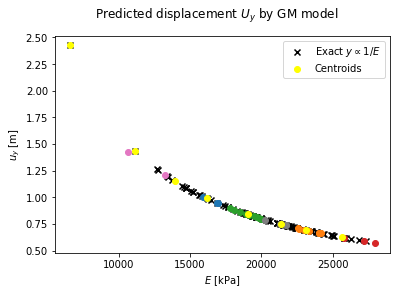
\includegraphics[width=\textwidth]{graphs/E_single/bayes_inversion_model_fit_view.png}
	\caption{Plot of the predicted output grouped by each cluster.}
	\end{subfigure}
	\begin{subfigure}{.45\textwidth}
	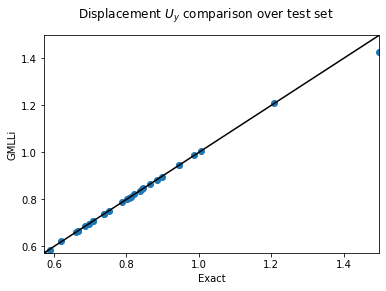
\includegraphics[width=\textwidth]{graphs/E_single/bayes_inversion_test_fit.png}
	\caption{Predicted output as function of real model output taken for the same input samples.}
	\end{subfigure}
	\caption{Fit of $\mathcal{M}(E) \propto 1/E$ using \texttt{GLLiM} method ($K=8$). 30 test samples are used to compare the exact method outputs to the surrogate predictions.}
	\end{figure}
	\end{frame}
	
	\begin{frame}{SSB: inversion of uniform young modulus.}
	\begin{figure}
	\begin{subfigure}{0.40\textwidth}
	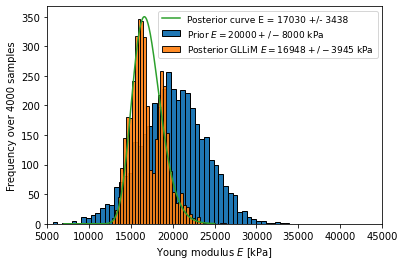
\includegraphics[width=\textwidth]{graphs/E_single/bayes_inversion_disc=0.1.png}
	\caption{$\sigma = 0.1 \si{m}$, $10\%$}
	\end{subfigure}
	\begin{subfigure}{0.40\textwidth}
	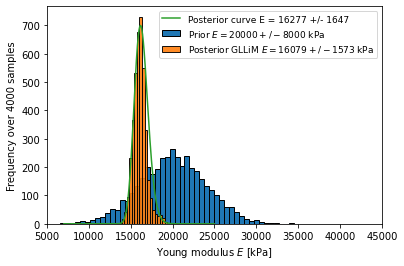
\includegraphics[width=\textwidth]{graphs/E_single/bayes_inversion_disc=0.05.png}
	\caption{$\sigma = 0.05 \si{m}$, $5\%$}
	\end{subfigure}
	
	\begin{subfigure}{0.40\textwidth}
	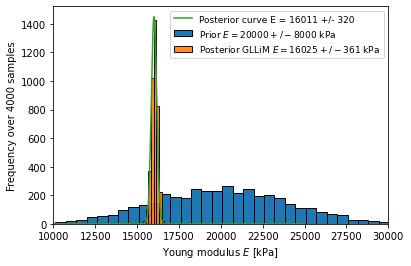
\includegraphics[width=\textwidth]{graphs/E_single/bayes_inversion_disc=0.01.png}
	\caption{$\sigma = 0.01 \si{m}$, $1\%$}
	\end{subfigure}
	%\caption{Plot of posterior distribution of $E$ taken over different discrepancies.}
	\end{figure}
	\end{frame}
	
	\begin{frame}{SSB: inversion of uniform young modulus.}
	\begin{figure}
	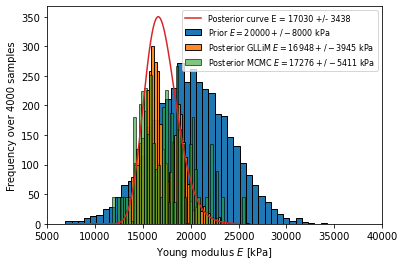
\includegraphics[width=0.8\textwidth]{graphs/E_single/bayes_inversion_disc=0.1_all.png}
	\caption{Comparison between \texttt{MCMC}, \texttt{GLLiM} and the \textcolor{red}{analytical posterior curve}.}
	\end{figure}
	\end{frame}
	
	\begin{frame}{SSB: inversion of uniform young modulus.}
	\begin{figure}
	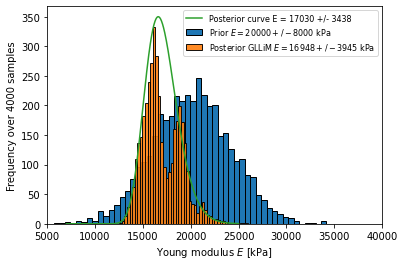
\includegraphics[width=0.8\textwidth]{graphs/E_single/bayes_inversion_disc=0.1_gllim.png}
	\caption{Comparison between \texttt{GLLiM} and the \textcolor{green}{analytical posterior curve}.}
	\end{figure}
	\end{frame}
	
	\begin{frame}{SSB: inversion of random field young modulus.}
	\begin{block}{System setup}
	\begin{itemize}
	\item Midpoint logNormal RF young modulus $E$, degree $M = 50$.
	\item Exponential correlation function with length $l_x = 0.5 \si{m}$.
	\item $E_{prior} = 20000 \pm 4000 \; \si{kPa}$.
	\item Measurement: at the center of the bar, $u_y(x=L/2) = 1.0 \si{m} \pm 0.1$.
	\end{itemize}
	\end{block}
	\begin{block}{Model $\mathcal{M} : \mathbb{R}^{50} \rightarrow \mathbb{R}$}
	\begin{itemize}
	\item \texttt{ZSoil} evaluated with continuum elements.
	\item Measurement: $u_y(x=L/2) = 1 \implies E = 16000 \; \si{kPa}$.
	\item GLLiM fitted, $K = 11$.
	\end{itemize}
	\end{block}
	\end{frame}
	
	\begin{frame}{SSB: inversion of LogNormal Random Field .}
	\begin{figure}
	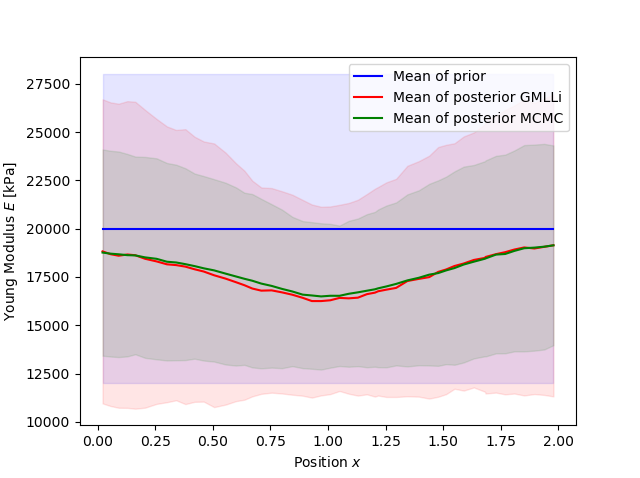
\includegraphics[width=0.75\textwidth]{graphs/rf_E/young_map.png}
	\caption{Random field mean and confidence interval ($2\times$ std. dev.) visualized for prior and posterior distribution over the spatial coordinate $x$.}
	\end{figure}
	\end{frame}
	
	\begin{frame}{SSB: inversion of LogNormal Random Field .}
	\begin{figure}
	\begin{subfigure}{0.48\textwidth}
	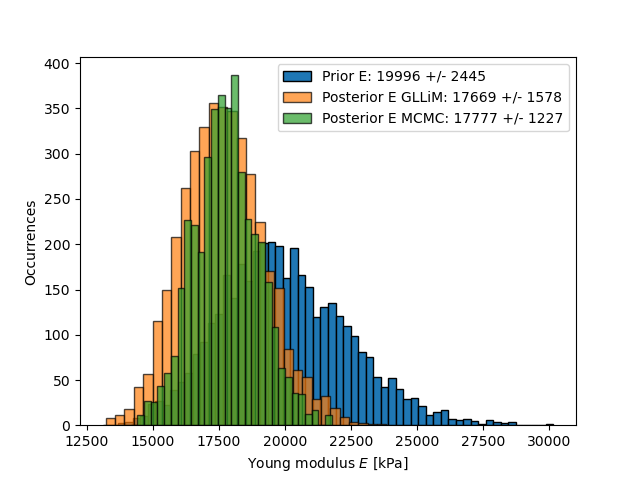
\includegraphics[width=\textwidth]{graphs/rf_E/young_hist.png}
	\caption{Spatial mean of prior vs. posterior RF, $\bar{E}_{post} = 17712 \pm 3000$.}
	\end{subfigure}
	\begin{subfigure}{0.48\textwidth}
	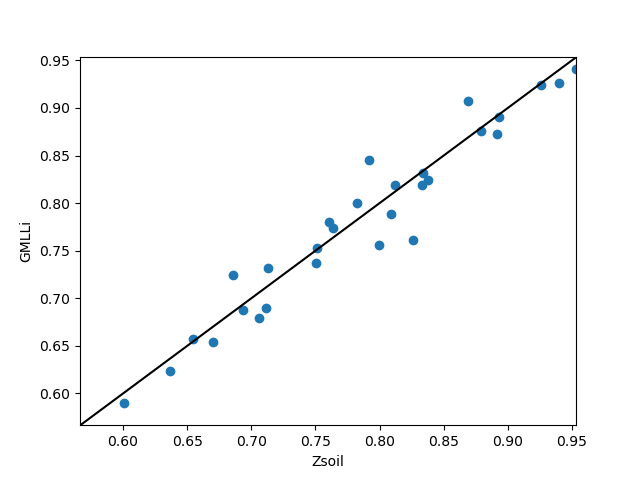
\includegraphics[width=\textwidth]{graphs/rf_E/gllim_test.png}
	\caption{Gaussian mixture mapping fit performance over test set.}
	\end{subfigure}
	\end{figure}
	\end{frame}
	
	\section{Conclusion}
	
	\begin{frame}{The point}
	\begin{block}{Attended goals}
	\begin{itemize}
	\item RF approximation with Midpoint
	\item Uncorrelated RF workflow
	\item PCE and PCK study
	\item Bayes inversion of a RF using \texttt{MCMC}: metropolis algorithm. 
	\item Implementation of fit and bayes inversion using \texttt{GMLLi}.
	\end{itemize}
	\end{block}
	
	\begin{block}{Final goals}
	\begin{itemize}
	\item Reduce number of variables to invert: K.L. RF.
	\item Code random fields cross correlation after inversion
	\item Deploy Python modules and separe them from tests
	\item Data augmentation with PCE/PCK?
	\end{itemize}
	\end{block}
	\end{frame}